\documentclass[11pt,oneside]{article}
\usepackage[T1]{fontenc}
\usepackage[utf8]{inputenc}
% \usepackage{lmodern}
%\usepackage[adobe-utopia,uppercase=upright,greeklowercase=upright]{mathdesign}
\usepackage[adobe-utopia]{mathdesign}
%\usepackage{minionpro}
% \usepackage{pifont}
% \usepackage{amssymb}
\usepackage{amsmath}
\usepackage[francais]{babel}
% \usepackage[francais]{varioref}
\usepackage[dvips]{graphicx}

\usepackage{framed}
\usepackage[normalem]{ulem}
\usepackage{fancyhdr}
\usepackage{titlesec}
\usepackage{vmargin}
\usepackage{longtable}

\usepackage{ifthen}


%\usepackage{epsfig}
\usepackage{subfig}

\usepackage{multirow}
\usepackage{multicol} % Portions de texte en colonnes
\usepackage{flafter}%floatants après la référence



\usepackage{color}
\usepackage{colortbl}


\definecolor{gris25}{gray}{0.75}
\definecolor{bleu}{RGB}{18,33,98}
\definecolor{bleuf}{RGB}{42,94,171}
\definecolor{bleuc}{RGB}{231,239,247}
\definecolor{rougef}{RGB}{185,18,27}
\definecolor{rougec}{RGB}{255,230,231}
\definecolor{vertf}{RGB}{103,126,82}
\definecolor{vertc}{RGB}{220,255,191}

\newenvironment{rem}[1][\hsize]%
{%
    \def\FrameCommand
    {%
\rotatebox{90}{\textit{\textsf{Remarque}}} 
        {\color{bleuf}\vrule width 3pt}%
        \hspace{0pt}%must no space.
        \fboxsep=\FrameSep\colorbox{bleuc}%
    }%
    \MakeFramed{\hsize#1\advance\hsize-\width\FrameRestore}%
}%
{\endMakeFramed}%


\newenvironment{savoir}[1][\hsize]%
{%
    \def\FrameCommand
    {%
\rotatebox{90}{\textit{\textsf{Savoir}}} 
        {\color{bleuf}\vrule width 3pt}%
        \hspace{0pt}%must no space.
        \fboxsep=\FrameSep\colorbox{bleuc}%
    }%
    \MakeFramed{\hsize#1\advance\hsize-\width\FrameRestore}%
}%
{\endMakeFramed}%

\newenvironment{prob}[1][\hsize]%
{%
    \def\FrameCommand%
    {%
\rotatebox{90}{\textit{\textsf{ Problématique}}} 
        {\color{rougef}\vrule width 3pt}%
        \hspace{0pt}%must no space.
        \fboxsep=\FrameSep\colorbox{rougec}%
    }%
    \MakeFramed{\hsize#1\advance\hsize-\width\FrameRestore}%
}%
{\endMakeFramed}%

\newenvironment{obj}[1][\hsize]%
{%
    \def\FrameCommand%
    {%
\rotatebox{90}{\textit{\textsf{ $\;$}}} 
        {\color{rougef}\vrule width 3pt}%
        \hspace{0pt}%must no space.
        \fboxsep=\FrameSep\colorbox{rougec}%
    }%
    \MakeFramed{\hsize#1\advance\hsize-\width\FrameRestore}%
}%
{\endMakeFramed}%

\newenvironment{defi}[1][\hsize]%
{%
    \def\FrameCommand%
    {%
\rotatebox{90}{\textit{\textsf{Définition\\}}} 
        {\color{bleuf}\vrule width 3pt}%
        \hspace{0pt}%must no space.
        \fboxsep=\FrameSep\colorbox{bleuc}%
    }%
    \MakeFramed{\hsize#1\advance\hsize-\width\FrameRestore}%
}%
{\endMakeFramed}%


\newenvironment{hypo}[1][\hsize]%
{%
    \def\FrameCommand%
    {%
\rotatebox{90}{\textit{\textsf{Hypothèse\\}}} 
        {\color{bleuf}\vrule width 3pt}%
        \hspace{0pt}%must no space.
        \fboxsep=\FrameSep\colorbox{bleuc}%
    }%
    \MakeFramed{\hsize#1\advance\hsize-\width\FrameRestore}%
}%
{\endMakeFramed}%


\newenvironment{prop}[1][\hsize]%
{%
    \def\FrameCommand%
    {%
\rotatebox{90}{\textit{\textsf{Propriété\\}}} 
        {\color{bleuf}\vrule width 3pt}%
        \hspace{0pt}%must no space.
        \fboxsep=\FrameSep\colorbox{bleuc}%
    }%
    \MakeFramed{\hsize#1\advance\hsize-\width\FrameRestore}%
}%
{\endMakeFramed}%

\newenvironment{props}[1][\hsize]%
{%
    \def\FrameCommand%
    {%
\rotatebox{90}{\textit{\textsf{Propriétés\\}}} 
        {\color{bleuf}\vrule width 3pt}%
        \hspace{0pt}%must no space.
        \fboxsep=\FrameSep\colorbox{bleuc}%
    }%
    \MakeFramed{\hsize#1\advance\hsize-\width\FrameRestore}%
}%
{\endMakeFramed}%

\newenvironment{exemple}[1][\hsize]%
{%
    \def\FrameCommand%
    {%
\rotatebox{90}{\textit{\textsf{Exemple\\}}} 
        {\color{vertf}\vrule width 3pt}%
        \hspace{0pt}%must no space.
        \fboxsep=\FrameSep\colorbox{vertc}%
    }%
    \MakeFramed{\hsize#1\advance\hsize-\width\FrameRestore}%
}%
{\endMakeFramed}%

\newenvironment{resultat}[1][\hsize]%
{%
    \def\FrameCommand%
    {%
\rotatebox{90}{\textit{\textsf{Résultat\\}}} 
        {\color{rougef}\vrule width 3pt}%
        \hspace{0pt}%must no space.
        \fboxsep=\FrameSep\colorbox{rougec}%
    }%
    \MakeFramed{\hsize#1\advance\hsize-\width\FrameRestore}%
}%
{\endMakeFramed}%

\newenvironment{methode}[1][\hsize]%
{%
    \def\FrameCommand%
    {%
\rotatebox{90}{\textit{\textsf{Méthode\\}}} 
        {\color{rougef}\vrule width 3pt}%
        \hspace{0pt}%must no space.
        \fboxsep=\FrameSep\colorbox{rougec}%
    }%
    \MakeFramed{\hsize#1\advance\hsize-\width\FrameRestore}%
}%
{\endMakeFramed}%

\newenvironment{theo}[1][\hsize]%
{%
    \def\FrameCommand%
    {%
\rotatebox{90}{\textit{\textsf{Théorème\\}}} 
        {\color{rougef}\vrule width 3pt}%
        \hspace{0pt}%must no space.
        \fboxsep=\FrameSep\colorbox{rougec}%
    }%
    \MakeFramed{\hsize#1\advance\hsize-\width\FrameRestore}%
}%
{\endMakeFramed}%

\newenvironment{warn}[1][\hsize]%
{%
    \def\FrameCommand%
    {%
\rotatebox{90}{\textit{\textsf{Attention\\}}} 
        {\color{rougef}\vrule width 3pt}%
        \hspace{0pt}%must no space.
        \fboxsep=\FrameSep\colorbox{rougec}%
    }%
    \MakeFramed{\hsize#1\advance\hsize-\width\FrameRestore}%
}%
{\endMakeFramed}%

% \usepackage{pstricks}
%\usepackage{minitoc}
% \setcounter{minitocdepth}{4}

\setcounter{tocdepth}{2}

% \mtcselectlanguage{french} 

%\usepackage{draftcopy}% "Brouillon"
% \usepackage{floatflt}
\usepackage{psfrag}
%\usepackage{listings} % Permet d'insérer du code de programmation
\renewcommand{\baselinestretch}{1.2}

% Changer la numérotation des figures :
% ------------------------------------
% \makeatletter
% \renewcommand{\thefigure}{\ifnum \c@section>\z@ \thesection.\fi
%  \@arabic\c@figure}
% \@addtoreset{figure}{section}
% \makeatother
 


%%%%%%%%%%%%
% Définition des vecteurs %
%%%%%%%%%%%%
 \newcommand{\vect}[1]{\overrightarrow{#1}}

%%%%%%%%%%%%
% Définition des torseusr %
%%%%%%%%%%%%

 \newcommand{\torseur}[1]{%
\left\{{#1}\right\}
}

\newcommand{\torseurcin}[3]{%
\left\{\mathcal{#1} \left(#2/#3 \right) \right\}
}

\newcommand{\torseurstat}[3]{%
\left\{\mathcal{#1} \left(#2\rightarrow #3 \right) \right\}
}

 \newcommand{\torseurc}[8]{%
%\left\{#1 \right\}=
\left\{
{#1}
\right\}
 = 
\left\{%
\begin{array}{cc}%
{#2} & {#5}\\%
{#3} & {#6}\\%
{#4} & {#7}\\%
\end{array}%
\right\}_{#8}%
}

 \newcommand{\torseurcol}[7]{
\left\{%
\begin{array}{cc}%
{#1} & {#4}\\%
{#2} & {#5}\\%
{#3} & {#6}\\%
\end{array}%
\right\}_{#7}%
}

 \newcommand{\torseurl}[3]{%
%\left\{\mathcal{#1}\right\}_{#2}=%
\left\{%
\begin{array}{l}%
{#1} \\%
{#2} %
\end{array}%
\right\}_{#3}%
}

 \newcommand{\vectv}[3]{%
\vect{V\left( {#1} \in {#2}/{#3}\right)}
}


\newcommand{\vectf}[2]{%
\vect{R\left( {#1} \rightarrow {#2}\right)}
}

\newcommand{\vectm}[3]{%
\vect{\mathcal{M}\left( {#1}, {#2} \rightarrow {#3}\right)}
}


 \newcommand{\vectg}[3]{%
\vect{\Gamma \left( {#1} \in {#2}/{#3}\right)}
}

 \newcommand{\vecto}[2]{%
\vect{\Omega\left( {#1}/{#2}\right)}
}
% }$$\left\{\mathcal{#1} \right\}_{#2} =%
% \left\{%
% \begin{array}{c}%
%  #3 \\%
%  #4 %
% \end{array}%
% \right\}_{#5}}

%  ------------------------------------------
% | Modification du formatage des sections : | 
%  ------------------------------------------

% Grands titres :
% ---------------

\newcommand{\titre}[1]{%
\begin{center}
      \bigskip
      \rule{\textwidth}{1pt}
      \par\vspace{0.1cm}
      
      \textbf{\large #1}
      \par\rule{\textwidth}{1pt}
    \end{center}
    \bigskip
  }

% Supprime le numéro du chapitre dans la numérotation des sections:
% -----------------------------------------------------------------
\makeatletter
\renewcommand{\thesection}{\@arabic\c@section}
\makeatother


% \titleformat{\chapter}[display]
% {\normalfont\Large\filcenter}
% {}
% {1pc}
% {\titlerule[1pt]
%   \vspace{1pc}%
%   \Huge}[\vspace{1ex}%
% \titlerule]


%%%% Chapitres Comme PY Pechard %%%%%%%%%
% numéro du chapitre
\DeclareFixedFont{\chapnumfont}{OT1}{phv}{b}{n}{80pt}
% pour le mot « Chapitre »
\DeclareFixedFont{\chapchapfont}{OT1}{phv}{m}{it}{40pt}
% pour le titre
\DeclareFixedFont{\chaptitfont}{T1}{phv}{b}{n}{25pt}

\definecolor{gris}{gray}{0.75}
\titleformat{\chapter}[display]%
	{\sffamily}%
	{\filleft\chapchapfont\color{gris}\chaptertitlename\
	\\
	\vspace{12pt}
	\chapnumfont\thechapter}%
	{16pt}%
	{\filleft\chaptitfont}%
	[\vspace{6pt}\titlerule\titlerule\titlerule]

%%%%  Fin Chapitres Comme PY Pechard %%%%%%%%%


% Section, subsection, subsubsection sans serifs :
% % ----------------------------------------------

% \makeatletter
% \renewcommand{\section}{\@startsection{section}{0}{0mm}%
% {\baselineskip}{.3\baselineskip}%
% {\normalfont\sffamily\Large\textbf}}%
% \makeatother

\makeatletter
\renewcommand{\@seccntformat}[1]{{\textcolor{bleu}{\csname
the#1\endcsname}\hspace{0.5em}}}
\makeatother

\makeatletter
\renewcommand{\section}{\@startsection{section}{1}{\z@}%
                       {-4ex \@plus -1ex \@minus -.4ex}%
                       {1ex \@plus.2ex }%
                       {\normalfont\Large\sffamily\bfseries}}%
\makeatother
 
\makeatletter
\renewcommand{\subsection}{\@startsection {subsection}{2}{\z@}
                          {-3ex \@plus -0.1ex \@minus -.4ex}%
                          {0.5ex \@plus.2ex }%
                          {\normalfont\large\sffamily\bfseries}}
\makeatother
 
\makeatletter
\renewcommand{\subsubsection}{\@startsection {subsubsection}{3}{\z@}
                          {-2ex \@plus -0.1ex \@minus -.2ex}%
                          {0.2ex \@plus.2ex }%
                          {\normalfont\large\sffamily\bfseries}}
\makeatother
 
\makeatletter             
\renewcommand{\paragraph}{\@startsection{paragraph}{4}{\z@}%
                                    {-2ex \@plus-.2ex \@minus .2ex}%
                                    {0.1ex}%               
{\normalfont\sffamily\bfseries}}
\makeatother
 
\makeatletter
\renewcommand{\subparagraph}{\@startsection{subparagraph}{5}{\z@}%
                                       {-2ex \@plus-.1ex \@minus .2ex}%
                                       {0.1ex}%
				    {\normalfont\normalsize\sffamily\bfseries}}
\makeatletter
% \makeatletter
% \renewcommand{\subsection}{\@startsection{subsection}{1}{2mm}%
% {\baselineskip}{.3\baselineskip}%
% {\normalfont\sffamily\large\textbf}}%
% \makeatother
% 
% \makeatletter
% \renewcommand{\subsubsection}{\@startsection{subsubsection}{2}{4mm}%
% {\baselineskip}{.15\baselineskip}%
% {\normalfont\sffamily\large\textbf}}%
% \makeatother
% 
% \makeatletter
% \renewcommand{\paragraph}{\@startsection{paragraph}{3}{6mm}%
% {\baselineskip}{.15\baselineskip}%
% {\normalfont\sffamily\large\textbf}}%
% \makeatother
 
\setcounter{secnumdepth}{4}


%  --------
% | Marges |
%  --------


% \setmarginsrb{2.5cm}{1.5cm}{2.5cm}{2cm}{1cm}{1cm}{1cm}{1cm}
\setmarginsrb{1.5cm}{1cm}{1cm}{1.5cm}{1cm}{1cm}{1cm}{1cm}

% Changer les marges localement :
% -----------------------------
\newenvironment{changemargin}[2]{\begin{list}{}{%
\setlength{\topsep}{0pt}%
\setlength{\leftmargin}{0pt}%
\setlength{\rightmargin}{0pt}%
\setlength{\listparindent}{\parindent}%
\setlength{\itemindent}{\parindent}%
\setlength{\parsep}{0pt plus 1pt}%
\addtolength{\leftmargin}{#1}%
\addtolength{\rightmargin}{#2}%
}\item }{\end{list}}



\usepackage{pst-solides3d}
\usepackage{titletoc}
\titlecontents{chapter}[+3pc]
  {\addvspace{10pt}\sffamily\bfseries}
{\contentslabel[{\pscirclebox[fillstyle=solid,fillcolor=gray!25,
linecolor=gray!25,framesep=4pt]{\textcolor{white}{\thecontentslabel}}}]{2.5pc}}
  {}
  {\dotfill \normalfont\thecontentspage\ }

\titlecontents{section}[3pc]
  {\addvspace{2pt}\sffamily}
  {\contentslabel[\thecontentslabel]{1.8pc}}
  {}
  {\dotfill \normalfont\thecontentspage\ }

\titlecontents{subsection}[5pc]
  {\addvspace{2pt}\sffamily}
  {\contentslabel[\thecontentslabel]{1.8pc}}
  {}
  {\dotfill \normalfont\thecontentspage\ }

\titlecontents{subsubsection}[8pc]
  {\addvspace{2pt}\sffamily}
  {\contentslabel[\thecontentslabel]{3pc}}
  {}
  {\dotfill \normalfont\thecontentspage\ }
%{\;\titlerule\;\normalfont\thecontentspage\ }

\titlecontents{paragraph}[9pc]
  {\addvspace{2pt}\sffamily}
  {\contentslabel[\thecontentslabel]{3.5pc}}
  {}
  {\dotfill \normalfont\thecontentspage\ }



\usepackage[raccourcis]{FAST}
\usepackage[%
    pdftitle={Produits Procédés Matériaux -- },
    pdfauthor={Xavier Pessoles},
    colorlinks=true,
    linkcolor=blue,
    citecolor=magenta]{hyperref}

\usepackage{pifont}


% \makeatletter \let\ps@plain\ps@empty \makeatother
%% DEBUT DU DOCUMENT
%% =================
\sloppy
\hyphenpenalty 10000

\newcommand{\Pointilles}[1][3]{%
\multido{}{#1}{\makebox[\linewidth]{\dotfill}\\[\parskip]
}}


\colorlet{shadecolor}{orange!15}

\newtheorem{theorem}{Theorem}


\begin{document}


\newboolean{prof}
\setboolean{prof}{true}
%------------- En tetes et Pieds de Pages ------------
\pagestyle{fancy}
\renewcommand{\headrulewidth}{0pt}

\fancyhead{}
\fancyhead[L]{%
\noindent\noindent\begin{minipage}[c]{2.6cm}
%Lycée Rouvière PTSI

\includegraphics[width=2cm]{png/logo_ptsi.png}%
\end{minipage}
}

\fancyhead[C]{\rule{12cm}{.5pt}}

\fancyhead[R]{%
\noindent\begin{minipage}[c]{3cm}
\begin{flushright}
\footnotesize{\textit{\textsf{Sciences Industrielles\\ pour l'Ingénieur}}}%
\end{flushright}
\end{minipage}
}

\renewcommand{\footrulewidth}{0.2pt}

\fancyfoot[C]{\footnotesize{\bfseries \thepage}}
\fancyfoot[L]{\footnotesize{2012 -- 2013} \\ X. \textsc{Pessoles}}
\ifthenelse{\boolean{prof}}{%
\fancyfoot[R]{\footnotesize{Cours -- CI 6 : PPM -- P}}
}{%
\fancyfoot[R]{\footnotesize{Cours -- CI 6 : PPM}}
}



\begin{center}
 \huge\textsc{CI 6 -- PPM -- Produits Procédés Matériaux}

 \large\textsc{Élaboration des pièces mécaniques. Introduction de la chaîne numérique.}
\end{center}

\begin{center}
 \LARGE\textsc{Chapitre 8 -- Cotation fonctionnelle}
\end{center}

%\begin{flushright}
%\textit{D'après documents de Jean-Pierre Pupier}
%\end{flushright}

\vspace{.5cm}



%\begin{minipage}[c]{.3\linewidth}
%\begin{center}
%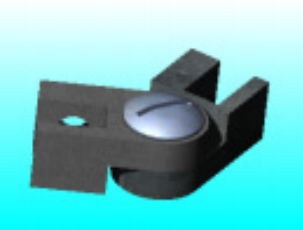
\includegraphics[height=2.5cm]{png/charniere1}

%\textit{Produit désiré par l'utilisateur}
%\end{center}
%\end{minipage} \hfill
%\begin{minipage}[c]{.3\linewidth}
%\begin{center}
%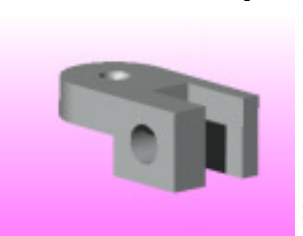
\includegraphics[height=2.5cm]{png/charniere2}

%\textit{Produit issu de la conception}
%\end{center}
%\end{minipage} \hfill
%\begin{minipage}[c]{.3\linewidth}
%\begin{center}
%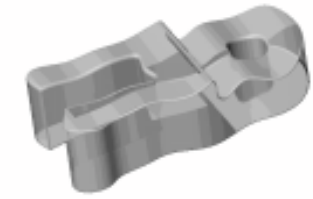
\includegraphics[height=2.5cm]{png/charniere3}

%\textit{Produit issu de la fabrication}
%\end{center}
%\end{minipage}

%\vspace{.5cm}



%\begin{center}
%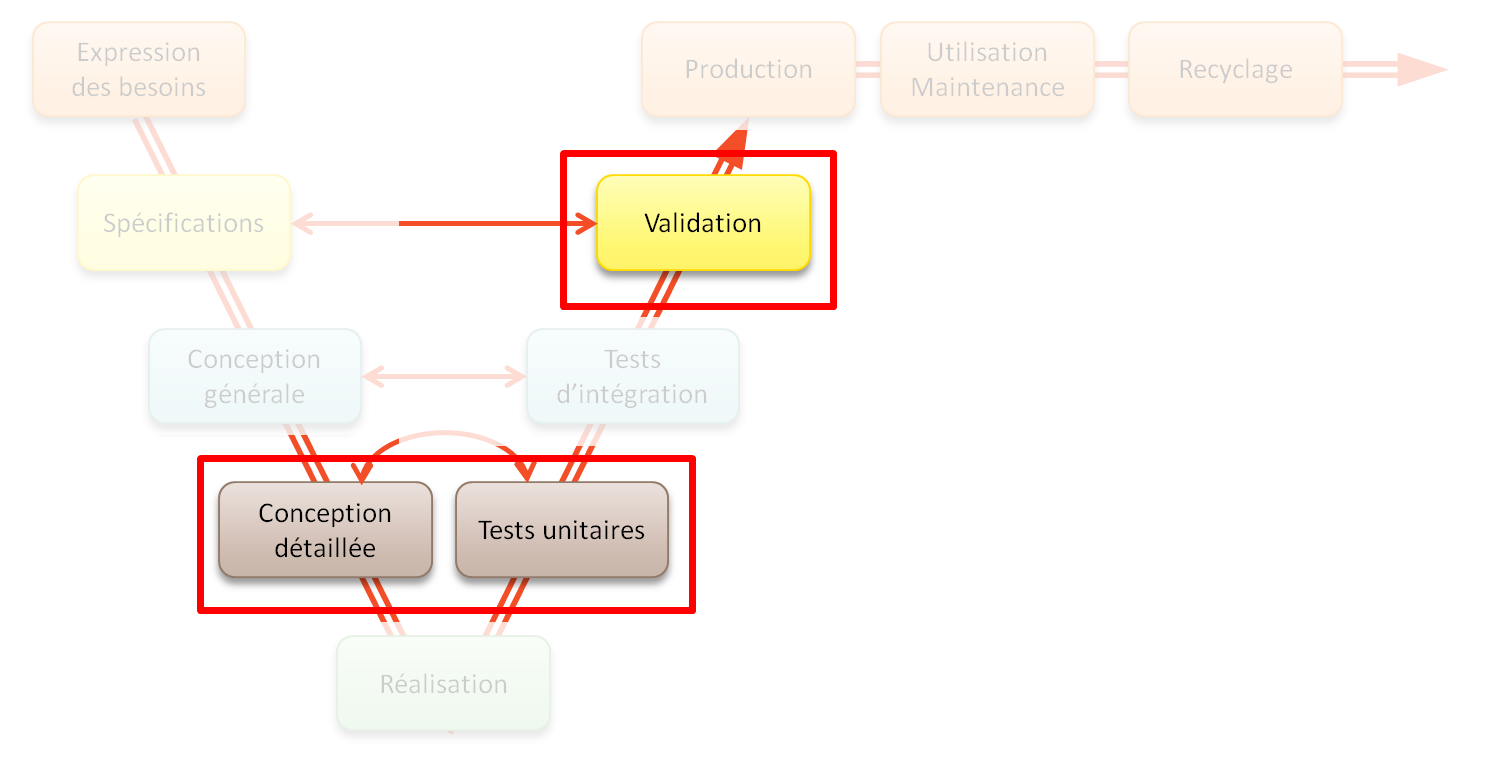
\includegraphics[width=.9\textwidth]{png/cyclev.png}

%\textit{Cycle de conception d'un produit}
%\end{center}

Les premiers exemples de conception laissent paraître qu'il est parfois nécessaire de laisser paraître des jeux fonctionnels afin de garantir le fonctionnement des systèmes. Dans un premier temps ce cours va permettre de visualiser l'influence des dimensions des différentes pièces sur les jeux. 

Dans un second temps on cherchera à réaliser les dessins de définition de différentes pièces en s'appuyant sur un cahier des charges. 

\begin{prob}
\textsc{Problématique :}
\begin{itemize}
\item Quelles sont les conditions fonctionnelles permettant le fonctionnement du système ?
\item Quelle est la chaîne de côte unidirectionnelle correspondant à une condition donnée ?
\end{itemize}
\end{prob}



\begin{savoir}
\textit{La cotation fonctionnelle est au programme de PT}

\textsc{Savoirs :}
\begin{itemize}
\item Conditions fonctionnelles d'aptitude à l'emploi
\item Cotation des cônes
\item Chaînes de cotes linéaires unidirectionnelle, suivant l'exigence de l'enveloppe, choix de la répartition des tolérances par la méthode iso qualité pour les pièces fabriquées
\end{itemize}
\end{savoir}
 

\setlength{\parskip}{0ex plus 0.2ex minus 0ex}
 \renewcommand{\contentsname}{}
 \renewcommand{\baselinestretch}{1}

\tableofcontents

 \renewcommand{\baselinestretch}{1.2}
\setlength{\parskip}{2ex plus 0.5ex minus 0.2ex}

% \vspace{1cm}
\textit{Ce document évolue. Merci de signaler toutes erreurs ou coquilles.}

\section{Les chaînes de cotes \cite{cf}}
\subsection{Les cotes conditions}
En fonction des exigences fonctionnelles, il peut être nécessaire d'exprimer des cotes conditions. Ici, le vecteur $\vect{J}$ exprime une exigence fonctionnelle. Cette cote fonctionnelle est limitée par deux éléments appelés surfaces terminales. Les surfaces de contact entre les pièces sont appelées surfaces de liaison. Lorsque la cote condition est positive, on parle de \textbf{jeu}. Dans le cas contraire on parle de \textbf{serrage}.

\begin{center}
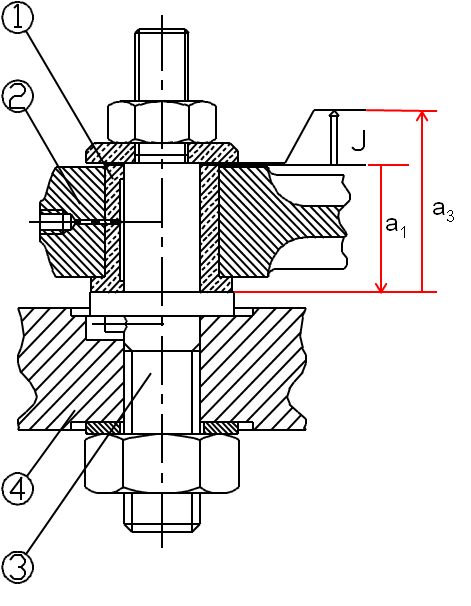
\includegraphics[width=.4\textwidth]{png/assemblage}
\end{center}

Par convention, la cote condition est représentée par un double trait. Les cotes conditions horizontales seront dirigées de gauche à droite et les cotes conditions verticales de haut en bas. 

Ici, pour permettre d'assurer la liaison pivot entre l'arbre 3 et la bielle 2, l'écrou ne doit pas venir appuyer sur la bielle. Le jeu $J=||\vect{J}||$ doit donc être positif.


\subsection{Les chaînes de cotes}

Une chaîne de cote est un ensemble de cotes nécessaires et suffisantes au respect de la cote condition. Dans l'exemple ci-dessus, le jeu ne doit pas dépasser une valeur limite au delà de laquelle le mouvement axial du palier 1 deviendrait trop important. 

\begin{resultat}
Voici quelques règles simples qui s'appliquent à la construction des chaînes de cotes. La chaîne de cotes débute à l'origine du vecteur condition et se termine à son extrémité, de sorte que :

$$\vect{J}=\vect{a_1}+\vect{a_3}$$

\begin{enumerate}
\item chaque cote de la chaîne, commence et se termine sur la même pièce. Le problème initial est de coter les différentes pièces du mécanisme;
\item il ne peut y avoir qu'une seule cote par pièce dans une même chaîne de cotes. La chaîne de cotes doit être la plus courte possible, afin de faire intervenir le moins de cotes possible. Si deux cotes de la chaîne appartiennent à la même pièce, c'est qu'il existe une chaîne de cotes encore plus courte réalisant le même vecteur condition ;
\item le passage d'une cote de la chaîne à la suivante se fait par la surface d'appui entre les deux pièces cotées. En effet, la fermeture vectorielle exprimée plus haut n'a de sens que si les origines des différents ai correspondent aux extrémités du $a_j$ précédent. La relation vectorielle écrite plus haut conduit en projection, aux relations suivantes :
\begin{itemize}
\item $J=a_1-a_3$ pour les cotes nominales;
\item $J_{maxi}=a_{1 maxi}-a_{3 mini}$ et $J_{mini}=a_{1 mini}-a_{3 maxi}$ pour les conditions extrêmes.
\end{itemize}
La différence entre les deux dernières équations conduit à la relation sur les intervalles de tolérance :
$$
IT_j = IT_{a_1}+IT_{a_3} 
$$
\item la somme des intervalles de tolérance des cotes intervenant dans une chaîne de cotes est égale à l'intervalle de tolérance de la cote condition. Cette propriété impose de choisir pour les cotes conditions de IT les plus larges possibles, afin de réduire le coût des pièces entrant dans la constitution de la chaîne.
\end{enumerate}
\end{resultat}

\begin{center}
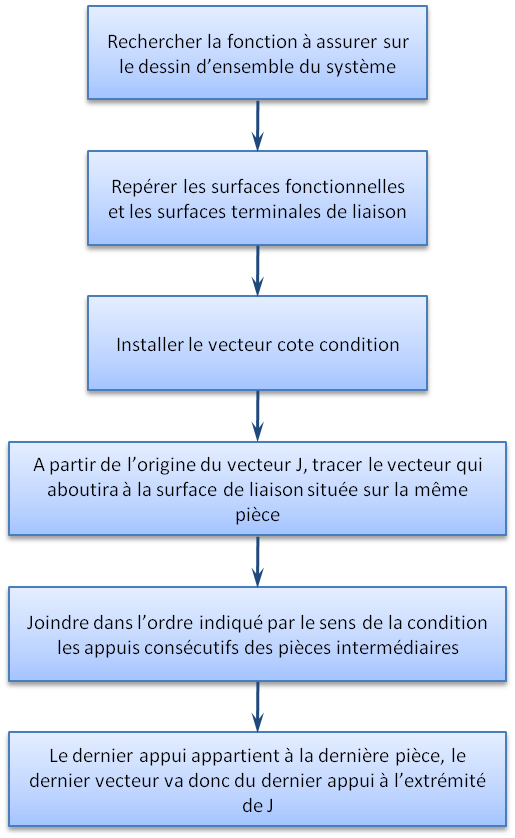
\includegraphics[width=.4\textwidth]{png/methode}
\end{center}

\subsection{Exemple d'application}
\subsubsection{Articulation vis axe}
\begin{itemize}
\item Tracez les chaînes de cotes installant les conditions JA et JB.
\item Inscrivez sur les dessins de définition, les cotes fonctionnelles relatives aux conditions indiquées ci-dessus.
\end{itemize}
 
\begin{center}
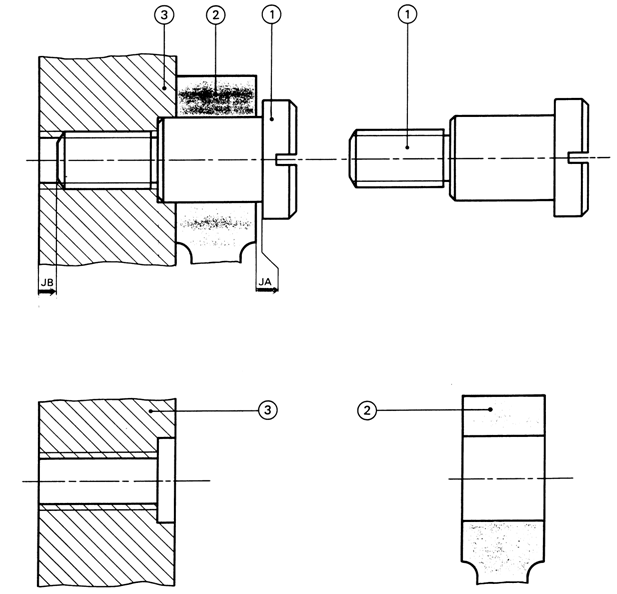
\includegraphics[width=.8\textwidth]{png/visaxe}
\end{center}
 
\newpage

\subsubsection{Guidage en rotation}
\begin{itemize}
\item Tracez les chaînes de cotes installant les conditions JA et JB.
\item Inscrivez sur les dessins de définition, les cotes fonctionnelles relatives aux conditions indiquées ci-dessus.
\end{itemize}
 

\begin{center}
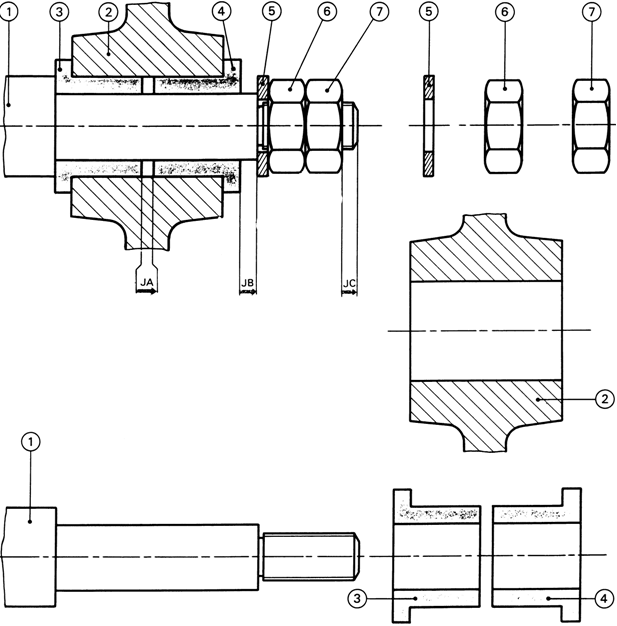
\includegraphics[width=.8\textwidth]{png/guidage}
\end{center}
 
\newpage

\subsubsection{Cotation comparée}
\begin{itemize}
\item Installez les conditions JA, etc...
\item Inscrivez les cotes fonctionnelles relatives à ces conditions sur les axes.
\item Comparez la cotation.
\end{itemize}

\begin{center}
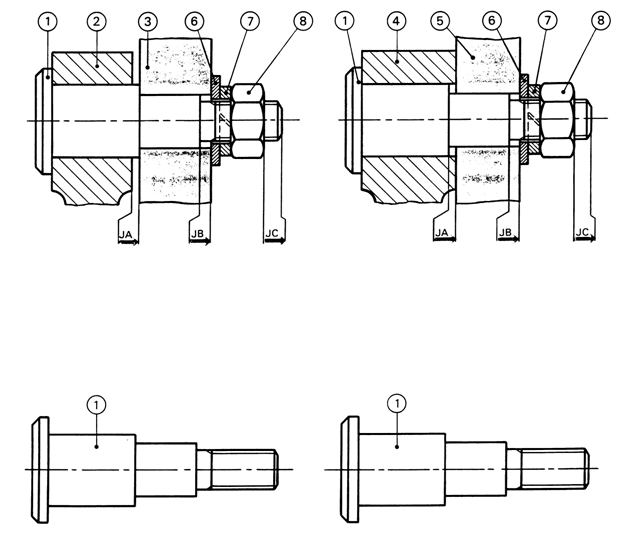
\includegraphics[width=.8\textwidth]{png/comparee}
\end{center}


\section{Cotation fonctionnelle d'un micromoteur}

\subsection{Mise en situation}
On donne le dessin d'ensemble d'un micromoteur associé à un cahier des charges partiel.

\begin{center}
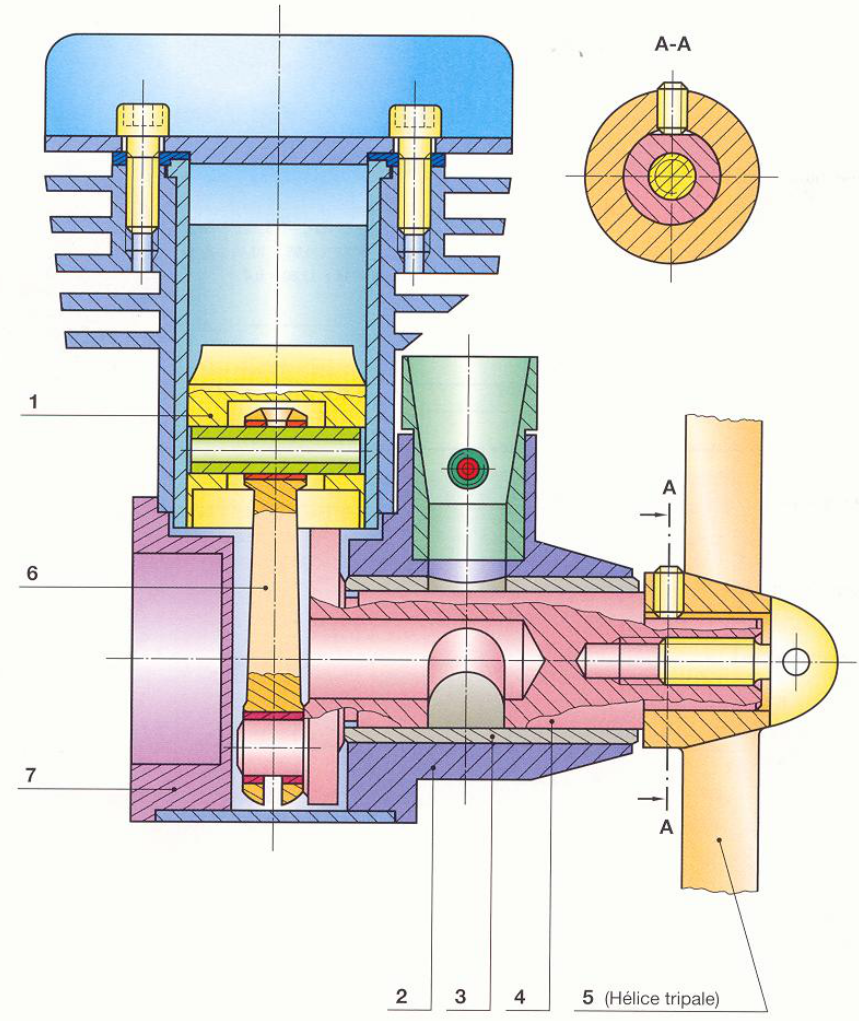
\includegraphics[width=.8\textwidth]{png/MicroMoteur}
\end{center}

\begin{center}
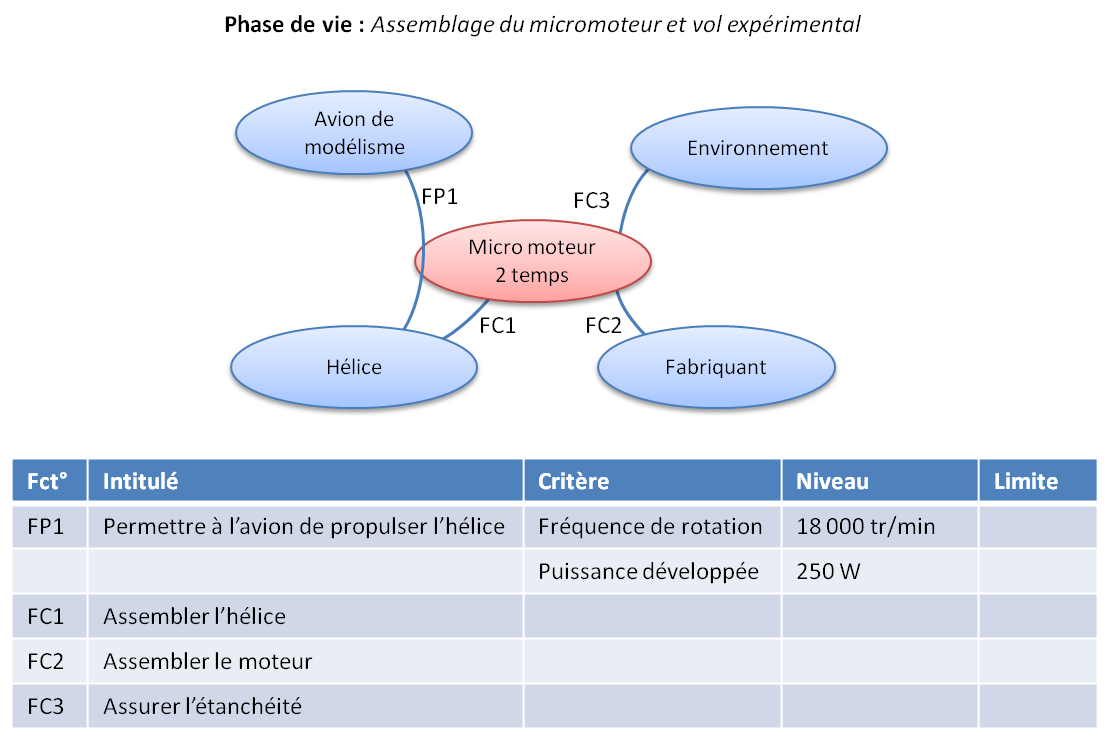
\includegraphics[width=.8\textwidth]{png/AF_MicroMoteur}
\end{center}

\begin{center}
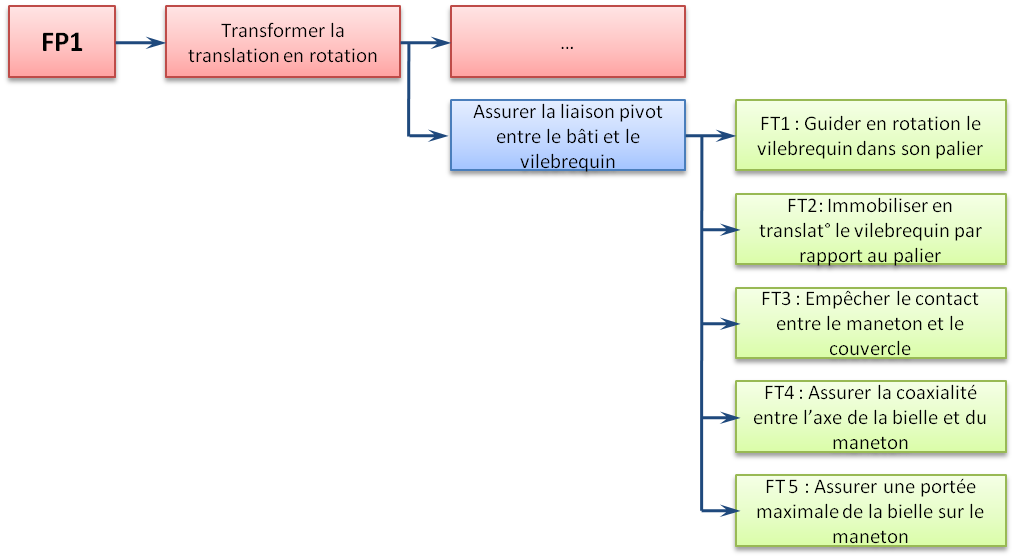
\includegraphics[width=.8\textwidth]{png/FAST_MicroMoteur}
\end{center}

\subsection{Réalisation des chaînes de cotes}
\textbf{
\begin{enumerate}
\item Tracer les chaînes de cotes associées à chacune des fonctions techniques.
\item Donner les relations permettant de déterminer le jeu mini et le jeu maxi pour chacune de ces chaînes de cotes.
\end{enumerate}}

\textit{Certains jeux ont été volontairement exagérés.}

\begin{center}
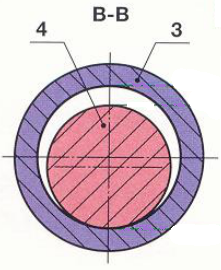
\includegraphics[width=.2\textwidth]{png/coupe}
\end{center}

\vspace{1cm}

\begin{center}
\includegraphics[width=.8\textwidth]{png/vilebrequin}
\end{center}

\vspace{1cm}

\begin{center}
\includegraphics[width=.8\textwidth]{png/vilebrequin}
\end{center}


\newpage
\subsection{Réalisation des dessins de définition}
 
\subsubsection{Le vilebrequin}
Une partie des exigences concourant au bon fonctionnement du mécanisme conduit à imposer :
\begin{itemize}
\item une spécification par dimension portant sur le diamètre du tourillon (grand diamètre) de vilebrequin;
\item une spécification par zone de tolérance portant sur la forme du tourillon;
\item une spécification par zone de tolérance portant sur la position du maneton par rapport au tourillon.
\end{itemize}

\begin{enumerate}
\item Préciser les fonctions qui seront réalisées grâce aux spécifications mentionnées ci-dessus
\item Porter ces spécifications sur le dessin de définition suivant.
\end{enumerate}

\begin{center}
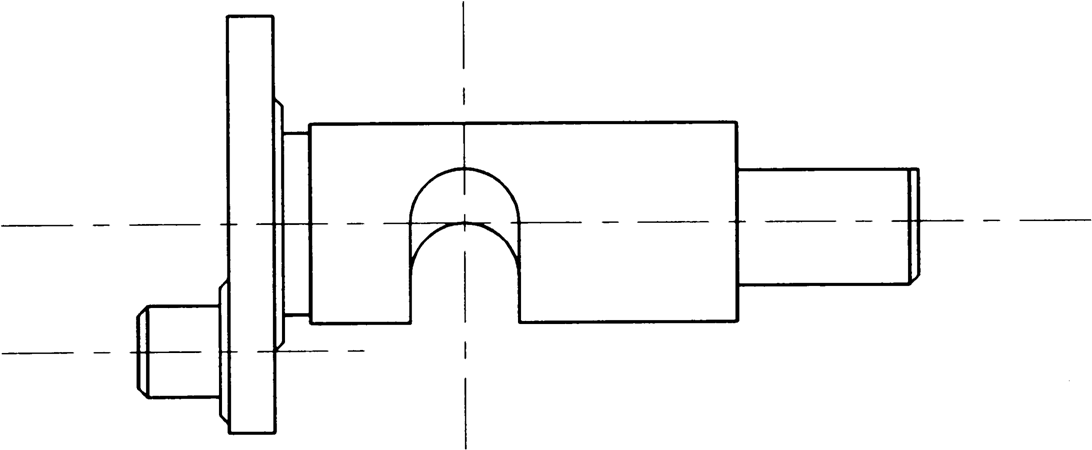
\includegraphics[width=.8\textwidth]{png/vilebrequin2}
\end{center}

\newpage
\subsubsection{Carter}
Parmi toutes les exigences permettant un coulissement satisfaisant du piston dans le cylindre chemisé on retiendra pour le moment celles liées à la qualité de la liaison entre cylindre et carter. Ce dernier est monobloc.

Ainsi :
\begin{itemize}
\item une première spécification définira le tolérancement de forme de la face d’appui du cylindre sur le carter;
\item une seconde spécification définira le tolérancement d’orientation de cette face d’appui par rapport à l’alésage recevant le coussinet guidant le tourillon de vilebrequin;
\item une troisième spécification définira le tolérancement de position de cette face par rapport à ce même alésage.
\end{itemize}

\begin{enumerate}
\item Préciser les fonctions qui seront réalisées grâce aux spécifications mentionnées ci-dessus.
\item Porter ces spécifications sur le dessin de définition suivant.
\end{enumerate}


\begin{center}
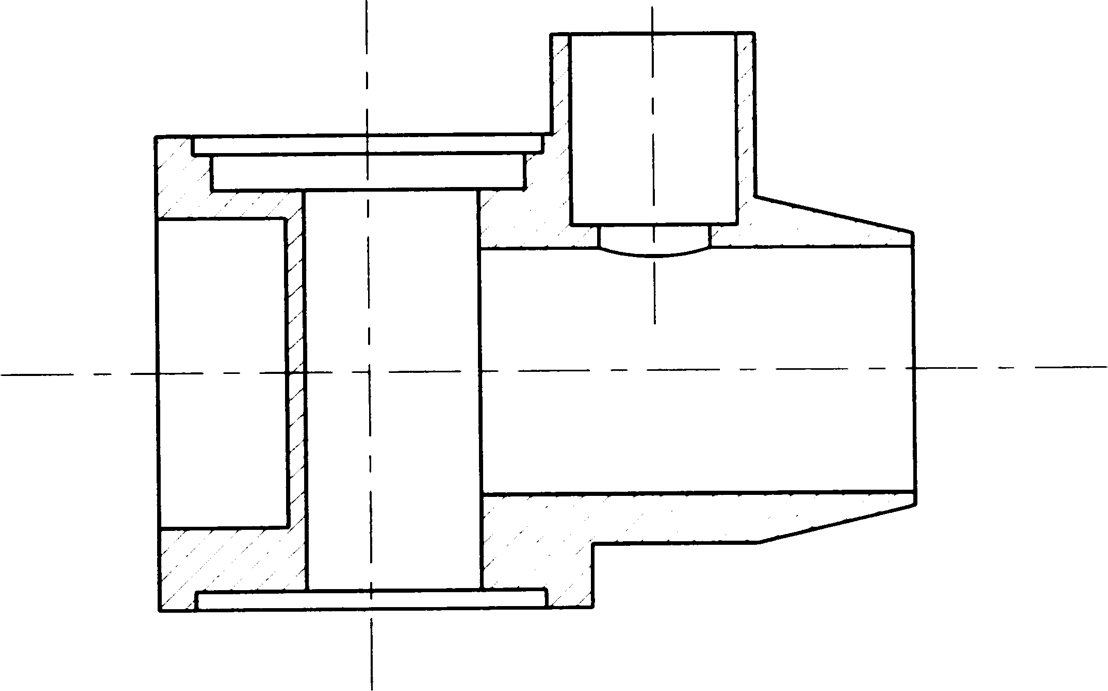
\includegraphics[width=.8\textwidth]{png/carter}
\end{center}

\newpage
 
\subsubsection{Le cylindre}
En gardant le même objectif d’un coulissement parfait du piston dans le cylindre chemisé, on se propose de définir une première spécification portant sur l’orientation de l’alésage recevant la chemise par rapport à la face d’appui du cylindre sur le carter.

De plus la culasse est centrée dans la chemise puis fixée sur le cylindre par quatre vis. En conséquence, une seconde spécification s’attache à exprimer la localisation des quatre trous taraudés permettant l’implantation de ces vis dans le cylindre.

\begin{enumerate}
\item Préciser les fonctions qui seront réalisées grâce aux spécifications mentionnées ci-dessus.
\item Porter ces spécifications sur le dessin de définition suivant.
\end{enumerate}


\begin{center}
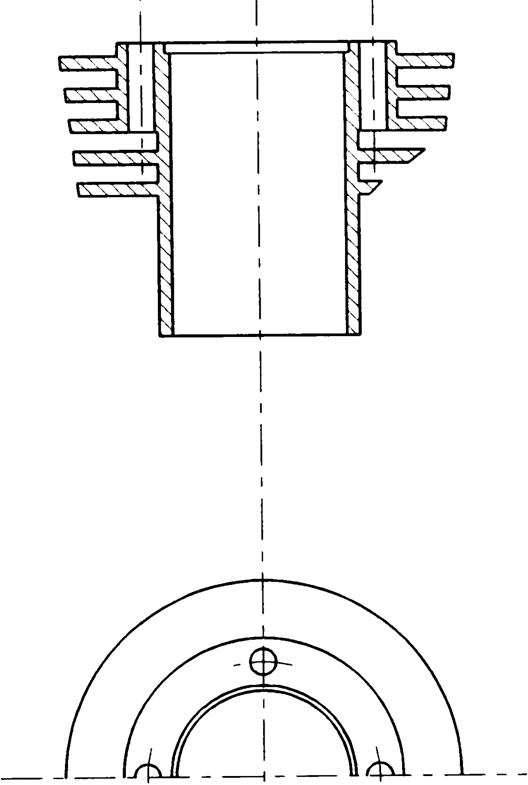
\includegraphics[width=.55\textwidth]{png/cylindre}
\end{center}

\newpage
\subsubsection{Bielle}
Le caractère hyperstatique de la chaîne cinématique cylindre, piston, bielle, vilebrequin carter est flagrant. Il faut donc une géométrie soignée en association avec des jeux judicieusement quantifiés:
\begin{itemize}
\item une spécification par zone de tolérance exprimera l’orientation relative des alésages de la tête et du pied de bielle;
\item le respect du taux de compression impose une spécification portant sur l’entraxe de celle-ci;
\item on considérera que l’alésage de tête de bielle joue un rôle prioritaire dans la situation de la bielle dans le mécanisme.
\end{itemize}

\begin{enumerate}
\item Préciser les fonctions qui seront réalisées grâce aux spécifications mentionnées ci-dessus
\item Porter ces spécifications sur le dessin de définition suivant.
\end{enumerate}

\begin{center}
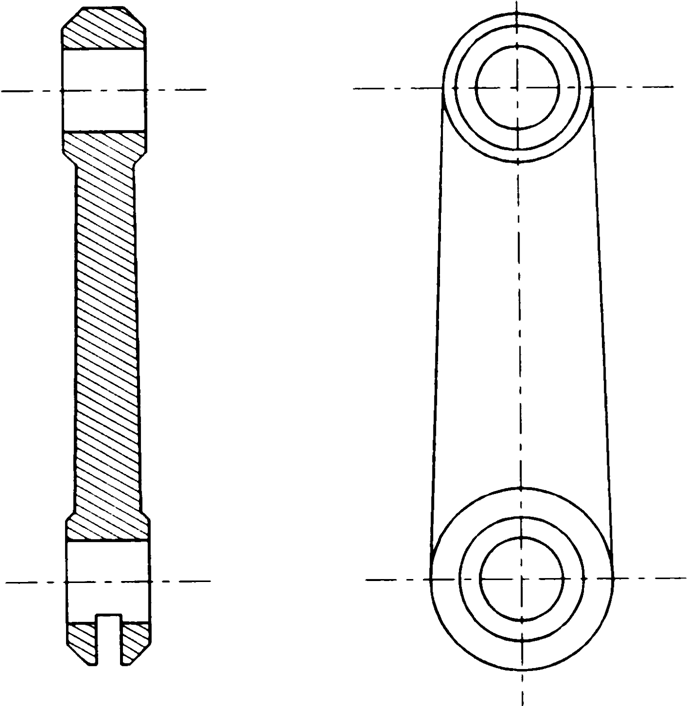
\includegraphics[width=.55\textwidth]{png/bielle}
\end{center}

\newpage
\subsubsection{Piston}
Les contraintes liées à la liaison pivot glissant établie entre piston et chemise sont nombreuses : 
\begin{itemize}
\item qualité du guidage;
\item étanchéité dynamique;
\item résolution de l’hyperstaticité.
\end{itemize}

Il faudra donc des spécifications par dimension, par zone de tolérance (forme et position).

\begin{enumerate}
\item Préciser les fonctions qui seront réalisées grâce aux spécifications mentionnées ci-dessus
\item Porter ces spécifications sur le dessin de définition suivant.
\end{enumerate}


\begin{center}
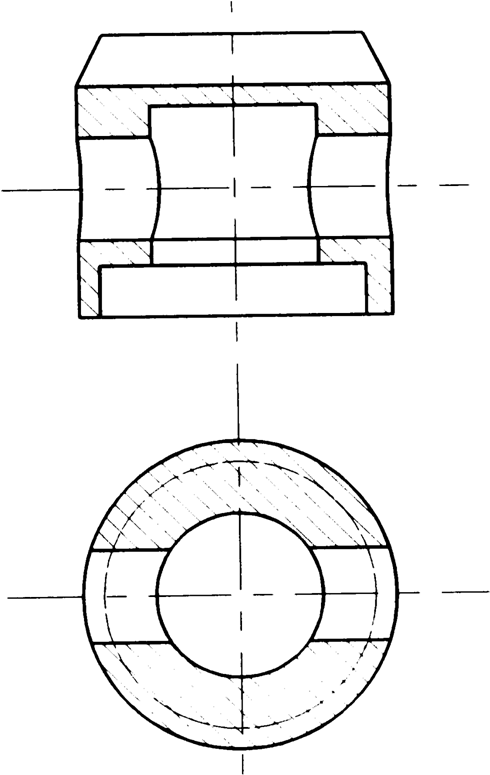
\includegraphics[width=.55\textwidth]{png/piston}
\end{center}


\begin{thebibliography}{2}
\bibitem{cf}{\textit{La cotation fonctionnelle}, PTSI -- Lycée Vauban, Brest.}
\bibitem{gdi}{\textit{Guide du dessinateur industriel}, André Chevalier, Éditions Hachette Technique, Editions 2004.}
\bibitem{jpp}{Supports de cours de Jean-Pierre Pupier, Lycée Rouvière, Toulon.}
%\bibitem{gps}{\textit{Centre d'Études et de Rénovation Pédagogique de l'Enseignement Technique}, Exploitation du concept G.P.S. et de la normalisation pour la Spécification Géométrique des Produits.}
%\bibitem{gps2}{\textit{Le Décodage du Dessin de Définition}, Guy Percebois, Lycée Louis Vincent -- Metz . \url{http://www.ac-nancy-metz.fr/enseign/sti/genimeca/zip/GPS/Tol\%20g\%E9o\%20pr\%E9\%20bac.pdf}}
%\bibitem{rb}{Supports de cours de Renan Bonnard,PTSI, Lycée Newton, Clichy la Garenne}
%\bibitem{jb}{Supports de cours de Joël Boiron, PTSI, Lycée Gustave Eiffel, Bordeaux}
%\bibitem{mc}{Supports de cours de Maryline Carrez, Lycée Jules Haag, Besançon}
%\bibitem{pf}{Supports de cours de Philippe Fichou, Lycée Vauban, Brest \url{http://philippe.fichou.pagesperso-orange.fr/documents/liaisoncomplete2003.pdf}}



\end{thebibliography}

\end{document}